\documentclass[10pt,a4paper]{article}
\usepackage[left=1.1cm,right=1.7cm,top=0.2cm,bottom=1.5cm]{geometry}
\usepackage{tikz}
\usepackage{listings}

\usepackage{xcolor}

\lstset
{
    language={[LaTeX]TeX},
    %alsolanguage={PGF/TikZ},
    frame=single,
    framesep=\fboxsep,
    framerule=\fboxrule,
    rulecolor=\color{red},
    xleftmargin=\dimexpr\fboxsep+\fboxrule,
    xrightmargin=\dimexpr\fboxsep+\fboxrule,
    breaklines=true,
    basicstyle=\small\tt,
    keywordstyle=\color{blue}\sf,
    identifierstyle=\color{magenta},
    commentstyle=\color{cyan},
    backgroundcolor=\color{yellow!10},
    tabsize=2,
    columns=flexible,
}

\begin{document}

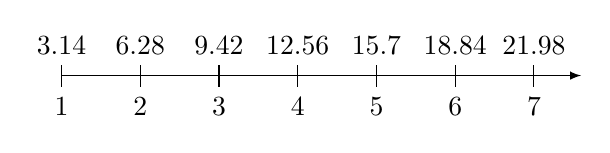
\begin{tikzpicture}

\foreach \x [count=\i] in {3.14,6.28,...,21.98} {
    \draw (\i,-4pt) -- (\i,4pt)
        node [below,yshift=-2ex] {\i}
        node [above] {\x};
}

\draw [-latex] (1,0) -- (7.6,0);

\end{tikzpicture}

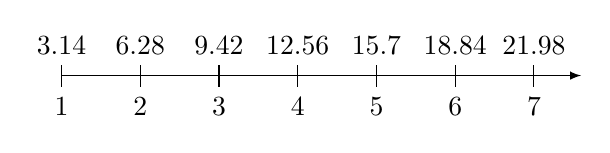
\begin{tikzpicture}

\foreach \i [evaluate=\i as \x using \i*3.14] in {1,2,...,7} {
    \draw (\i,-4pt) -- (\i,4pt)
        node [below,yshift=-2ex] {\i}
        node [above] {\x};
}

\draw [-latex] (1,0) -- (7.6,0);

\end{tikzpicture}


\begin{lstlisting}{LaTeX}
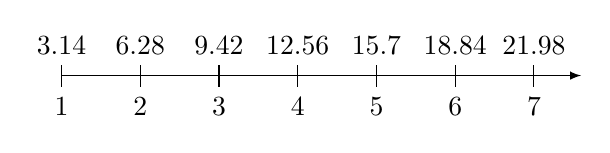
\begin{tikzpicture}

\foreach \x [count=\i] in {3.14,6.28,...,21.98} {
    \draw (\i,-4pt) -- (\i,4pt)
        node [below,yshift=-2ex] {\i}
        node [above] {\x};
}

\draw [-latex] (1,0) -- (7.6,0);

\end{tikzpicture}

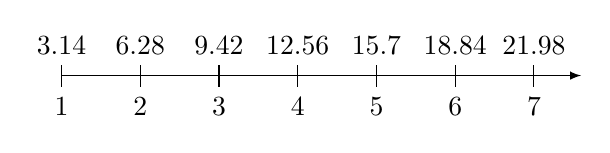
\begin{tikzpicture}

\foreach \i [evaluate=\i as \x using \i*3.14] in {1,2,...,7} {
    \draw (\i,-4pt) -- (\i,4pt)
        node [below,yshift=-2ex] {\i}
        node [above] {\x};
}

\draw [-latex] (1,0) -- (7.6,0);

\end{tikzpicture}

\end{lstlisting}


% Membuat jangka sorong
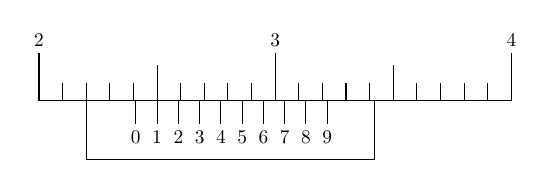
\begin{tikzpicture}[scale=3]
\draw[](2,0)--(4,0);
\draw (2.2,0) rectangle (3.42,-0.25);

\foreach \x in {2,3,4}{ \draw (\x,0) -- (\x,0.2)node[above,scale=0.7]{\x}; } \foreach \x in {2.1,2.2,...,4}{ \draw (\x,0) -- (\x,0.075); } \foreach \x in {2.5,3.5}{ \draw (\x,0) -- (\x,0.15); }

\foreach \x [evaluate=\x as \label using \x*0.09+2.41] in {0,1,...,9}
{ \draw (\label ,0) -- (\label ,-0.1)node[below,scale=0.7]{\x}; 
}
  \end{tikzpicture}
%------------listing ---------------------
\begin{lstlisting}{LaTeX}

% Membuat jangka sorong
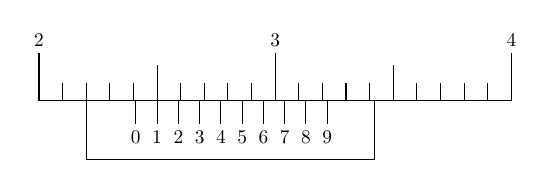
\begin{tikzpicture}[scale=3]
\draw[](2,0)--(4,0);
\draw (2.2,0) rectangle (3.42,-0.25);

\foreach \x in {2,3,4}{ \draw (\x,0) -- (\x,0.2)node[above,scale=0.7]{\x}; } \foreach \x in {2.1,2.2,...,4}{ \draw (\x,0) -- (\x,0.075); } \foreach \x in {2.5,3.5}{ \draw (\x,0) -- (\x,0.15); }

\foreach \x [evaluate=\x as \label using \x*0.09+2.41] in {0,1,...,9}
{ \draw (\label ,0) -- (\label ,-0.1)node[below,scale=0.7]{\x}; 
}
  \end{tikzpicture}
\end{lstlisting}

\end{document}
